% !TeX root = p2p.tex

\section{Project code overview} \label{sec:code}

\setminted[text]{breaklines, tabsize=2, xleftmargin=14pt}

The simulations were designed to work with the \emph{cycle-driven} engine of the \peersim{} \cite{peersim} simulator. This section explains how the protocol classes were adapted to comply to the synchronous communication model, and then illustrates the main features of the implemented protocols.

\subsection{Synchronous communication model}

Implementing the algorithms as cycle-driven protocols seems a natural choice given the assumption of synchronous communication under which the algorithms are specified: the cycle-driven engine simply iterates over each \texttt{Node} in the network array and executes the protocol logic at each step. However, to correctly model the synchronous communication, a protocol shouldn't be able to influence another one in the middle of a cycle, since if this happens while the second protocol is yet to be executed, it would receive information one cycle (or step) in advance. In other words, each protocol must be executed in isolation from the others at each cycle, and a message generated during a cycle should reach the destination only at the beginning of the following one.

To solve this issue, whenever a new message is generated it must be retained by the sender protocol until the iteration of the current cycle is finished, and then delivered to the receiver protocol. This can be achieved in a number of different ways; the choice made here was to define a generic interface providing methods to allow \emph{synchronous} protocols to communicate with each other under the requirement above but in a way that is transparent to the logic of the protocol itself, and defining a \peersim{} \texttt{Control} to move deliver messages at the end of each cycle.

\subsubsection{Components}

The \texttt{CycleBasedTransportSupport} interface is the generic interface that syn\-chro\-nous protocol classes are required to implement (its type argument is the class that models the messages protocols exchange with each other):
\begin{minted}[breaklines=false]{text}
public interface CycleBasedTransportSupport<T> {
  interface SendQueueEntry<T> {
      T getMessage();
      CycleBasedTransportSupport<T> getDestination();
  }
  void addToSendQueue(
      T message, CycleBasedTransportSupport<T> destination);
  boolean hasOutgoingMessages();
  void addToIncoming(T message);
  Iterator<T> getIncomingMessagesIterator();
  Iterator<SendQueueEntry<T>> getSendQueueIterator();
}
\end{minted}
A protocol invokes the \texttt{addToSendQueue} method to ``send'' a message to the specified \texttt{destination} argument. The message is not actually sent, but held in a container until the cycle ends and the \texttt{CycleBasedTransport} control begins the execution. The control then obtains an iterator to the send queue of each protocol (with the \texttt{getSendQueueIterator} method), and moves the messages to the destinations by calling the \texttt{addToIncoming} method on them with the messages as arguments. A protocol can access available messages by obtaining an \texttt{Iterator} over them with the \texttt{getIncomingMessagesIterator} method.

\subsection{Protocol classes}

\begin{figure}
\centering
%\includegraphics[width=0.72\textwidth]{diagram4.pdf}
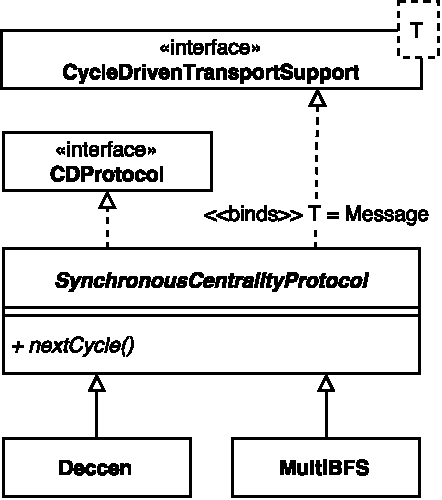
\includegraphics[height=0.31\textheight]{diagram_final.pdf}
\caption{Protocol classes.}
\label{class:protocol:hierarchy}
\end{figure}

Protocol classes are organized as shown in figure \ref{class:protocol:hierarchy}. Both \texttt{Deccen} and \texttt{MultiBFS} extend the abstract class \texttt{SynchronousCentralityProtocol}, which provides an implementation the \texttt{Cycle\-Based\-Transport\-Support<Message>} interface and declares the \texttt{nextCycle} method of the \texttt{CDProtocol} PeerSim interface \texttt{abstract}.

\subsubsection{Messages}
The messages exchanged by the protocols during the simulation are instances of the \texttt{Message} class. This class provides factory methods to generate \mdisc{} and \mrep{} message objects that follow the conventions used in the definition of the algorithms. 

\subsubsection{\deccen{} protocol implementation}

The \texttt{Deccen} class implements a \deccen{} node in the simulator. A node state consists of the shortest path information it collects and of the reports it has handled during the execution:
\begin{minted}{text}
public class Deccen extends SynchronousCentralityProtocol {
  private static class ShortestPathData {
    public final int count;
    public final int length;

    public ShortestPathData(int count, int length) { ... }
  }

  private static class OrderedPair<T1,T2> {
    public final T1 first;
    public final T2 second;

    public OrderedPair(T1 first, T2 second) { ... }
    ...
  }
  ...
  private Map<Node,ShortestPathData> shortestPathMap;
  private Set<OrderedPair<Long,Long>> handledReports;
  ...
  public void nextCycle(Node self, int protocolID) { ... }
  ...
}
\end{minted}
Whenever new \mdisc{} messages are received, additional information about the number and length of shortest paths toward a particular source becomes available: this information is stored in the \texttt{shortestPathMap} structure by adding a new \texttt{ShortestPathData} entry paired with the source of the discovery. Since the algorithm computes all the centrality indices, it stores both the distance from the source and the number of different paths counted. Reports about a source--destination pair $(s,t)$ are tracked by storing the \texttt{handledReports} set an \texttt{Ordered\-Pair} of \texttt{Node} IDs (which are \texttt{long} integers in \peersim{}).

The implementation of \texttt{nextCycle} simply executes the actions described in section \ref{deccen:step}:
\begin{minted}{text}
public void nextCycle(Node self, int protocolID) {
  Map<Node,List<Message>> discoveryMap =
      new HashMap<Node,List<Message>>();
  List<Message> reportList = new LinkedList<Message>();
  parseIncomingMessages(discoveryMap, reportList);
  if (!discoveryMap.isEmpty())
    processDiscoveryMessages(self, protocolID, discoveryMap);
  if (!reportList.isEmpty())
    processReportMessages(self, protocolID, reportList);
}
\end{minted}

\subsubsection{\multibfs{} protocol implementation}

The state of a \multibfs{} node consists of a \texttt{Map} to keep track of the various visits that are performed by the source nodes during the algorithm execution:

\begin{minted}{text}
public class MultiBFS extends SynchronousCentralityProtocol {
  private static class VisitState {
    ...
  }
  ...
  private Map<Node, VisitState> activeVisits;
  private Set<Node> completed;
  ...
  public void nextCycle(Node self, int protocolID) { ... }
  ...
  public boolean isWaiting(Node source) { ... }
  public boolean isActive(Node source) { ... }
  public boolean isCompleted(Node source) { ... }
}
\end{minted}
Recall that the state of a node is parametric with respect to each source of a visit. The state is \swait{\texttt{s}} if the \texttt{Node} instance \texttt{s} does not appear as key in the \texttt{activeVisits} map and neither is contained in the \texttt{completed} set; this is the initial state for any source since both structures are empty at the start of the protocol. When a node is in state \sact{\texttt{s}} an entry with key \texttt{s} is present in the \texttt{activeVisits} map. After a node has reported back to all the predecessors, it changes state \scomp{\texttt{s}} by removing the mapping from \texttt{activeVisits} and inserting \texttt{s} in the \texttt{completed} set.

Entries in the \texttt{activeVisits} map are used to store data while a node is in the ``active'' phase. A \texttt{VisitState} object is used to keep track of the predecessors and children sets, and to incrementally compute the values to be reported to the predecessor nodes:
\begin{minted}{text}
private static class VisitState {
  public Set<Node> predecessors;
  public Set<Node> siblings;
  public Set<Node> children;
  public int distanceFromSource;
  public int timestamp;
  public int sigma;
  public long contributionSC;
  public double contributionBC;
  ...	
  public void accumulate(
      Node child, double bcc, long scc, int numSP) { ... }
}
\end{minted}
The \texttt{accumulate} method updates the local contributions of the source by applying the recursive relations \eqref{eq:th:contrib:bc} and \eqref{eq:th:contrib:sc}, and it's invoked whenever a child node sends a report.

Finally, the \texttt{nextCycle} method follows the specification given in section \ref{multibfs:step}:
\begin{minted}{text}
public void nextCycle(Node self, int protocolID) {
  Map<Node,List<Message>> discoveryMap =
      new HashMap<Node,List<Message>>();
  List<Message> reportList = new LinkedList<Message>();
  parseIncomingMessages(discoveryMap, reportList);
  if (!discoveryMap.isEmpty())
    processDiscoveryMessages(self, protocolID, discoveryMap);
  if (!reportList.isEmpty())
    processReportMessages(reportList);
  reportNewCompleted(self, protocolID);
}
\end{minted}
Messages are parsed and handled by type, then active visits for which all child nodes have reported are finalized with the \texttt{reportNewCompleted} method by integrating the contributions in the centrality accumulators and reporting the relevant data to each predecessor.